\chapter{Electromagnetic Waves and the Maxwell Action}

\lectureoverview{We first solve the source-free Maxwell equations for a
plane wave and let the equations determine its polarization, field
geometry, and speed. We then ask a deeper question: which local,
Lorentz-invariant, gauge-invariant action produces the dynamical Maxwell
equations? The answer ties the electromagnetic field, charge
conservation, and gauge invariance into one structure.}

\section{Two Families of Maxwell Equations}

We begin with a plane electromagnetic wave. Here \emph{plane} is the
geometrical word, not \emph{plain} in the sense of unadorned. The
immediate questions are concrete: what does such a wave look like, and
how does its form follow from Maxwell's equations?

It is useful to put the equations into two columns before doing anything
with the wave. In empty space they are
\begin{align}
\nabla\cdot\mathbf B&=0,
&
\dot{\mathbf B}&=\nabla\times\mathbf E,
\label{eq:homogeneous-vector}
\\
\nabla\cdot\mathbf E&=0,
&
\dot{\mathbf E}&=-\,\nabla\times\mathbf B.
\label{eq:dynamical-vector-vacuum}
\end{align}
We use the mostly-plus metric
\begin{equation}
\eta_{\mu\nu}=\operatorname{diag}(-1,1,1,1)
\end{equation}
and the course convention
\begin{equation}
F_{\mu\nu}
=
\partial_\mu A_\nu-\partial_\nu A_\mu,
\qquad
F_{0i}=E_i,
\qquad
F_{ij}=\epsilon_{ijk}B_k.
\label{eq:course-f-convention}
\end{equation}
Then the same two families can be written
\begin{align}
\partial_\mu F_{\nu\sigma}
+\partial_\nu F_{\sigma\mu}
+\partial_\sigma F_{\mu\nu}
&=0,
\label{eq:bianchi-l9}
\\
\partial_\mu F^{\mu\nu}
&=0.
\label{eq:vacuum-maxwell-covariant}
\end{align}

\begin{figure}[H]
\centering

\includegraphics[width=\linewidth]{../../figures/lecture_09_figure_01.png}
\caption{The two vacuum Maxwell families and their covariant forms. The
cyclic equation is an identity; the contracted equation is dynamical.}
\par\smallskip
\textit{Lecture frame: 00:03:30.}
\end{figure}

The distinction between the two rows matters. Equation
\eqref{eq:bianchi-l9} follows identically from the existence of the
potential \(A_\mu\): every term is a second derivative, and the terms
cancel in pairs. It is therefore a Bianchi identity. Equation
\eqref{eq:vacuum-maxwell-covariant}, by contrast, is an equation of
motion. Change the electromagnetic Lagrangian and this is the family
that changes.

There is a small observation on the board that will do two jobs in this
chapter. Every field in Maxwell's equations appears differentiated.
That fact will constrain the relative phases of a plane wave, and it will
later make gauge invariance natural.

\section{A Plane Wave Along the \texorpdfstring{\(z\)}{z}-Axis}

Choose coordinates so that the wave propagates along the \(z\)-axis.
This costs no generality; a wave in another direction can be brought to
this form by rotating the axes. Let \(k\) be its wave number,
\begin{equation}
\lambda=\frac{2\pi}{k},
\end{equation}
and let \(\omega\) be its frequency. Before imposing any equation of
motion, write all six field components with a common phase
\begin{equation}
\theta=kz-\omega t:
\end{equation}
\begin{align}
E_x(z,t)&=\epsilon_x\sin\theta,
&
B_x(z,t)&=\beta_x\sin\theta,
\nonumber\\
E_y(z,t)&=\epsilon_y\sin\theta,
&
B_y(z,t)&=\beta_y\sin\theta,
\label{eq:plane-wave-ansatz}\\
E_z(z,t)&=\epsilon_z\sin\theta,
&
B_z(z,t)&=\beta_z\sin\theta.
\nonumber
\end{align}
The six Greek letters are constant amplitudes.

\begin{figure}[H]
\centering

\includegraphics[width=\linewidth]{../../figures/lecture_09_figure_02.png}
\caption{The six-component plane-wave ansatz before Maxwell's equations
remove the forbidden amplitudes.}
\par\smallskip
\textit{Lecture frame: 00:08:45.}
\end{figure}

Why begin with the same sinusoidal dependence for \(\mathbf E\) and
\(\mathbf B\)? Suppose one field carried \(\sin\theta\) and the other
carried \(\cos\theta\). A time derivative on one side of a curl equation
and a spatial derivative on the other would then produce different
trigonometric functions. The equality could not hold for every \(z\)
and \(t\). A common constant phase is allowed, but translating the
origin of \(z\) removes it. Thus the ansatz is not an extra dynamical
law; it is the simplest representative of the phase relation the
differential equations will require.

No Maxwell equation has yet been used. We have only chosen a direction,
a wavelength, and a convenient phase origin. The equations will now
decide which amplitudes survive.

\subsection{The divergence constraints}

Because the fields depend only on \(z\) and \(t\),
\begin{equation}
\nabla\cdot\mathbf E
=
\partial_xE_x+\partial_yE_y+\partial_zE_z
=
\partial_zE_z.
\end{equation}
In empty space this must vanish for every phase, so
\begin{equation}
\epsilon_z=0.
\label{eq:epsilon-z-zero}
\end{equation}
The identical argument for the magnetic field gives
\begin{equation}
\beta_z=0.
\label{eq:beta-z-zero}
\end{equation}
Neither field has a component along the direction of propagation. The
wave is transverse.

There remains a rotational freedom in the transverse \(xy\)-plane. The
pair \((\epsilon_x,\epsilon_y)\) is an ordinary two-dimensional vector,
so rotate the transverse axes until
\begin{equation}
\epsilon_y=0,
\qquad
\epsilon_x\ne0.
\label{eq:polarization-axis}
\end{equation}
This is a choice of linear polarization, not a restriction on the
physics.

\begin{figure}[H]
\centering

\includegraphics[width=\linewidth]{../../figures/lecture_09_figure_03.png}
\caption{The longitudinal amplitudes have vanished and the transverse
electric axis has been chosen.}
\par\smallskip
\textit{Lecture frame: 00:14:30.}
\end{figure}

\subsection{The curl equations}

Use the \(x\)-component of
\(\dot{\mathbf E}=-\nabla\times\mathbf B\). Since the fields vary only
with \(z\),
\begin{equation}
\dot E_x
=
-\left(\nabla\times\mathbf B\right)_x
=
\partial_zB_y.
\end{equation}
Substituting the ansatz gives
\begin{align}
-\omega\epsilon_x\cos\theta
&=
k\beta_y\cos\theta,
\nonumber\\
\beta_y
&=
-\,\epsilon_x\frac{\omega}{k}.
\label{eq:beta-y-epsilon}
\end{align}
The \(y\)-component of the same Maxwell equation reads
\begin{equation}
\dot E_y
=
-\left(\partial_zB_x\right).
\end{equation}
The left side is zero by our polarization choice, so
\begin{equation}
\beta_x=0.
\label{eq:beta-x-zero}
\end{equation}

\begin{figure}[H]
\centering

\includegraphics[width=\linewidth]{../../figures/lecture_09_figure_04.png}
\caption{A component curl calculation relates \(\epsilon_x\) to
\(\beta_y\) and removes the remaining magnetic amplitude.}
\par\smallskip
\textit{Lecture frame: 00:20:15.}
\end{figure}

The geometry is therefore fixed:
\begin{equation}
\mathbf E\parallel\hat{\mathbf x},
\qquad
\mathbf B\parallel\hat{\mathbf y},
\qquad
\mathbf k\parallel\hat{\mathbf z}.
\end{equation}
The electric field, magnetic field, and direction of travel are mutually
perpendicular.

\begin{figure}[H]
\centering

\includegraphics[width=0.94\linewidth]{../../figures/lecture_09_figure_05.png}
\caption{The board picture of the transverse electric and magnetic
oscillations advancing along the \(z\)-axis.}
\par\smallskip
\textit{Lecture frame: 00:23:15.}
\end{figure}

The other curl equation supplies an independent amplitude relation. Its
\(y\)-component is
\begin{equation}
\dot B_y=(\nabla\times\mathbf E)_y=\partial_zE_x,
\end{equation}
and therefore
\begin{align}
-\omega\beta_y\cos\theta
&=
k\epsilon_x\cos\theta,
\nonumber\\
\epsilon_x
&=
-\,\beta_y\frac{\omega}{k}.
\label{eq:epsilon-beta-y}
\end{align}

\begin{figure}[H]
\centering

\includegraphics[width=\linewidth]{../../figures/lecture_09_figure_06.png}
\caption{The reciprocal amplitude relations above the transverse-wave
sketch.}
\par\smallskip
\textit{Lecture frame: 00:25:00.}
\end{figure}

Combining equations \eqref{eq:beta-y-epsilon} and
\eqref{eq:epsilon-beta-y} gives the dispersion relation
\begin{equation}
\left(\frac{\omega}{k}\right)^2=1.
\end{equation}
For the positive-frequency wave moving in the chosen direction,
\begin{equation}
\omega=k
\qquad
(c=1).
\label{eq:omega-k}
\end{equation}
The common phase is consequently
\begin{equation}
\theta=k(z-t).
\end{equation}
Restoring ordinary units gives
\begin{equation}
\omega=ck,
\qquad
\theta=k(z-ct).
\label{eq:restore-c-wave}
\end{equation}
Thus the profile moves rigidly at the speed of light. In the units used
on the board, the electric and magnetic amplitudes have equal magnitude.
Their relative minus sign is an orientation convention: it says which
way the chosen \(y\)-axis points, not that one field lags the other by a
quarter cycle.

\begin{figure}[H]
\centering

\includegraphics[width=\linewidth]{../../figures/lecture_09_figure_07.png}
\caption{The final plane-wave form after \(\omega=k\) has been imposed.}
\par\smallskip
\textit{Lecture frame: 00:26:45.}
\end{figure}

\begin{classroomqa}
\audiencequestion{Do \(\omega\) and \(k\) not have different units?}
\lecturerresponse{They do in ordinary units: \(\omega\) is inverse time
and \(k\) is inverse length. With \(c=1\), time and length have the same
unit. Restoring \(c\) changes \(\omega=k\) into \(\omega=ck\), exactly as
dimensional analysis requires. \lecturetimestamp{00:25:55}}
\end{classroomqa}

\begin{classroomqa}
\audiencequestion{Are the electric and magnetic fields always in phase in
a plane wave?}
\lecturerresponse{They have the same phase dependence. Their signed
amplitudes can differ by a minus sign, which may be described as a
\(180^\circ\) reversal, but Maxwell's equations do not permit a
\(90^\circ\) sine--cosine lag for this linearly polarized plane wave.
Circular polarization is assembled from transverse components and
requires more careful language, but it does not alter this componentwise
Maxwell relation. \lecturetimestamp{00:27:31}}
\end{classroomqa}

\begin{classroomqa}
\audiencequestion{If both fields pass through zero together, is energy
still conserved?}
\lecturerresponse{Yes. The energy density at one fixed point oscillates
as the wave passes, but the energy has moved rather than disappeared.
What occupied one region at one time occupies a neighboring region a
moment later. Local energy transport, represented more fully by the
Poynting flux, reconciles the changing density with conservation.
\lecturetimestamp{00:28:15}}
\end{classroomqa}

Maxwell's equations are linear. The amplitude \(\epsilon_x\) may be
large or small, \(\beta_y\) follows from it, and any sum or difference of
solutions is again a solution. Waves traveling in different directions
may therefore be superposed. This brief calculation is worth doing:
an account of electromagnetism should not leave the electromagnetic wave
as an unexplained quotation.

\begin{classroomqa}
\audiencequestion{Did the derivation assume from the start that
\(\mathbf E\) and \(\mathbf B\) had the same phase?}
\lecturerresponse{The common phase was written as an ansatz, but it is
not an independent physical assumption. Because each side of the curl
equations differentiates a field, the equations eliminate a nontrivial
relative phase. A common phase shift can then be removed by translating
the origin. \lecturetimestamp{00:29:56}}
\end{classroomqa}

\begin{classroomqa}
\audiencequestion{Where did the second relation
\(\epsilon_x=-\beta_y\omega/k\) come from?}
\lecturerresponse{The first relation came from
\(\dot{\mathbf E}=-\nabla\times\mathbf B\). The second comes from the
companion equation \(\dot{\mathbf B}=\nabla\times\mathbf E\), with
\(\mathbf E\) and \(\mathbf B\) interchanged in the same component
calculation. Both are needed to obtain \(\omega^2=k^2\).
\lecturetimestamp{00:30:25}}
\end{classroomqa}

\section{Why Differential Equations Are Not Enough}

We now turn from a particular solution to the structure of the theory.
The principle of least action is what organizes energy conservation,
momentum conservation, and their relation to spacetime symmetries.
One can invent differential equations that possess no energy worth
calling conserved and no useful symmetry principle. Maxwell's equations
should instead arise from a Lagrangian.

Only the dynamical family needs to be produced:
\begin{equation}
\partial_\mu F^{\mu\nu}=J^\nu.
\label{eq:target-sourced-maxwell}
\end{equation}
The Bianchi family already follows from the definition of \(F_{\mu\nu}\).
In three-vector language, our convention makes
\begin{align}
\nabla\cdot\mathbf E&=\rho,
\label{eq:gauss-source}
\\
\dot{\mathbf E}+\nabla\times\mathbf B&=-\,\mathbf J.
\label{eq:ampere-course-sign}
\end{align}
The minus sign in \eqref{eq:ampere-course-sign} is important. It is the
component form of \eqref{eq:target-sourced-maxwell} under
\eqref{eq:course-f-convention}, and it will be rediscovered in a live
sign check near the end.

\begin{figure}[H]
\centering

\includegraphics[width=\linewidth]{../../figures/lecture_09_figure_08.png}
\caption{The full Maxwell board at the transition from the wave solution
to the action principle.}
\par\smallskip
\textit{Lecture frame: 00:32:45.}
\end{figure}

\section{Local Relativistic Field Theory}

The first principle is locality. An action is an integral over spacetime
of a density built from fields and their first derivatives at the same
point:
\begin{equation}
S=\int d^4x\,\mathcal L(\phi,\phi_{,\mu}),
\qquad
\phi_{,\mu}\equiv\partial_\mu\phi.
\label{eq:local-action}
\end{equation}
The comma is a compact derivative notation. The second principle is
Lorentz invariance: \(\mathcal L\) must be a scalar.

\subsection{A scalar-field rehearsal}

Before varying a four-vector, rehearse the method with one scalar field.
A local Lorentz scalar may depend on a potential \(U(\phi)\) and on the
contraction of two derivatives:
\begin{equation}
\mathcal L_\phi
=
-\frac12\,\partial_\mu\phi\,\partial^\mu\phi-U(\phi).
\label{eq:scalar-lagrangian}
\end{equation}
With the mostly-plus metric,
\begin{equation}
\partial_\mu\phi\,\partial^\mu\phi
=
-\dot\phi^{\,2}+|\nabla\phi|^2,
\end{equation}
so
\begin{equation}
\mathcal L_\phi
=
\frac12\dot\phi^{\,2}
-\frac12|\nabla\phi|^2
-U(\phi).
\end{equation}
The raised time derivative differs in sign from the lowered one; raised
and lowered spatial derivatives do not.

\begin{classroomqa}
\audiencequestion{Does it mean anything to put the derivative index
upstairs rather than downstairs?}
\lecturerresponse{Yes. Raising the index contracts with the inverse
metric. With signature \((-+++)\),
\(\partial^0=-\partial_0\) while
\(\partial^i=\partial_i\). That is why the time-derivative term carries
the opposite sign from the three spatial terms.
\lecturetimestamp{00:38:02}}
\end{classroomqa}

The field Euler--Lagrange equation is
\begin{equation}
\partial_\mu\left(
\frac{\partial\mathcal L}{\partial\phi_{,\mu}}
\right)
=
\frac{\partial\mathcal L}{\partial\phi}.
\label{eq:field-el}
\end{equation}
For \eqref{eq:scalar-lagrangian},
\begin{equation}
\frac{\partial\mathcal L_\phi}{\partial\phi_{,\mu}}
=
-\partial^\mu\phi,
\qquad
\frac{\partial\mathcal L_\phi}{\partial\phi}
=
-U'(\phi),
\end{equation}
and hence
\begin{equation}
\Box\phi=U'(\phi),
\qquad
\Box\equiv\partial_\mu\partial^\mu.
\end{equation}
Equivalently,
\begin{equation}
\ddot\phi-\nabla^2\phi=-U'(\phi).
\label{eq:scalar-wave}
\end{equation}
On the board only the \(x\)-derivative is written before the \(y\) and
\(z\) terms are left implicit. The result is the familiar wave equation
with a force from the potential.

\begin{figure}[H]
\centering

\includegraphics[width=\linewidth]{../../figures/lecture_09_figure_09.png}
\caption{Locality, a scalar Lorentz-invariant Lagrangian, and the
field-theory Euler--Lagrange equation.}
\par\smallskip
\textit{Lecture frame: 00:41:00.}
\end{figure}

The electromagnetic calculation is the same variational process with
four fields and more indices.

\section{Gauge Invariance Selects the Maxwell Scalar}

Add a third principle: gauge invariance. For the moment set
\(J^\mu=0\) and consider the free field. A gauge transformation is
\begin{equation}
A_\mu\longrightarrow A_\mu+\partial_\mu\chi.
\label{eq:gauge-transform}
\end{equation}
The field tensor does not change because mixed second derivatives
commute:
\begin{align}
F_{\mu\nu}
&\longrightarrow
F_{\mu\nu}
+\partial_\mu\partial_\nu\chi
-\partial_\nu\partial_\mu\chi
\nonumber\\
&=F_{\mu\nu}.
\end{align}

Lorentz invariance alone would allow the scalar
\begin{equation}
A_\mu A^\mu.
\end{equation}
It is nevertheless forbidden in Maxwell theory because it changes under
\eqref{eq:gauge-transform}. The indices in this expression label field
components; they are not derivatives. A derivative is indicated by a
comma, as in \(A_{\nu,\mu}=\partial_\mu A_\nu\).

\begin{figure}[H]
\centering

\includegraphics[width=\linewidth]{../../figures/lecture_09_figure_10.png}
\caption{The gauge transformation and the Lorentz scalar
\(A_\mu A^\mu\), which is rejected because it is not gauge invariant.}
\par\smallskip
\textit{Lecture frame: 00:43:40.}
\end{figure}

We should therefore build the free Lagrangian from \(F_{\mu\nu}\).
The linear trace fails:
\begin{equation}
F^\mu{}_\mu=0.
\end{equation}
Antisymmetry forces every diagonal component
\(F_{00},F_{11},F_{22},F_{33}\) to vanish. Raising an index may change a
sign, but it cannot turn zero into anything else.

\begin{figure}[H]
\centering

\includegraphics[width=\linewidth]{../../figures/lecture_09_figure_11.png}
\caption{The attempted linear trace and the vanishing diagonal entries of
the antisymmetric field tensor.}
\par\smallskip
\textit{Lecture frame: 00:47:00.}
\end{figure}

The first nonzero Lorentz scalar is quadratic:
\begin{equation}
F_{\mu\nu}F^{\mu\nu}.
\label{eq:f2-scalar}
\end{equation}
Let us unpack the contraction rather than quote it. The mixed components
contain the electric field. Raising their time index contributes a
minus sign, and both orderings \(0i\) and \(i0\) occur:
\begin{equation}
\sum_i\left(F_{0i}F^{0i}+F_{i0}F^{i0}\right)
=-2E^2.
\end{equation}
The purely spatial components contain the magnetic field. Raising
spatial indices changes no sign, and both orderings again occur:
\begin{equation}
\sum_{i<j}\left(F_{ij}F^{ij}+F_{ji}F^{ji}\right)
=2B^2.
\end{equation}
Therefore
\begin{equation}
F_{\mu\nu}F^{\mu\nu}=2(B^2-E^2),
\qquad
-F_{\mu\nu}F^{\mu\nu}=2(E^2-B^2).
\label{eq:f2-eb}
\end{equation}

\begin{figure}[H]
\centering

\includegraphics[width=\linewidth]{../../figures/lecture_09_figure_12.png}
\caption{The completed contraction in terms of electric and magnetic
field magnitudes.}
\par\smallskip
\textit{Lecture frame: 00:51:00.}
\end{figure}

\begin{classroomqa}
\audiencequestion{Is \(F_{00}\) also zero?}
\lecturerresponse{Yes. Every diagonal component of an antisymmetric
tensor vanishes, including \(F_{00}\). Only the off-diagonal mixed
components, which encode \(\mathbf E\), and the off-diagonal spatial
components, which encode \(\mathbf B\), contribute.
\lecturetimestamp{00:51:36}}
\end{classroomqa}

The conventional normalization is
\begin{equation}
\boxed{
\mathcal L_{\mathrm{EM}}
=
-\frac14F_{\mu\nu}F^{\mu\nu}
}
\label{eq:maxwell-lagrangian}
\end{equation}
or
\begin{equation}
\mathcal L_{\mathrm{EM}}
=
\frac12(E^2-B^2).
\label{eq:maxwell-lagrangian-eb}
\end{equation}
The minus sign gives the electric term the familiar positive sign. The
factor \(1/4\) compensates the twofold appearance of each antisymmetric
pair and leaves the conventional factor \(1/2\). Multiplying the entire
free action by a nonzero constant would not change its source-free
equations, but this normalization is the one that fits the standard
source coupling.

\section{Varying the Free Electromagnetic Field}

The independent fields are
\begin{equation}
A_0,\qquad A_x,\qquad A_y,\qquad A_z.
\end{equation}
For each component \(A_\nu\), the Euler--Lagrange equation is
\begin{equation}
\partial_\mu\left(
\frac{\partial\mathcal L}{\partial A_{\nu,\mu}}
\right)
=
\frac{\partial\mathcal L}{\partial A_\nu},
\qquad
A_{\nu,\mu}\equiv\partial_\mu A_\nu.
\label{eq:vector-el-comma}
\end{equation}
The placement in the comma notation is worth reading slowly: the first
index labels which component of \(A\) is the field; the second labels the
coordinate of differentiation.

In this notation,
\begin{equation}
F_{\mu\nu}
=
A_{\nu,\mu}-A_{\mu,\nu}.
\label{eq:f-comma-consistent}
\end{equation}
This is exactly \eqref{eq:course-f-convention}. Writing the comma indices
in the opposite verbal order changes an intermediate minus sign, which
is why a component calculation is useful.

\begin{figure}[H]
\centering

\includegraphics[width=\linewidth]{../../figures/lecture_09_figure_13.png}
\caption{The field tensor expressed in comma notation after the four
potential components have been identified as independent fields.}
\par\smallskip
\textit{Lecture frame: 00:55:30.}
\end{figure}

\begin{figure}[H]
\centering

\includegraphics[width=\linewidth]{../../figures/lecture_09_figure_14.png}
\caption{The Maxwell Lagrangian written explicitly in terms of derivatives
of the vector potential.}
\par\smallskip
\textit{Lecture frame: 00:56:45.}
\end{figure}

\subsection{One representative derivative}

Select the derivative \(A_{x,y}=\partial_yA_x\). The \(xy\) and \(yx\)
terms in the full sum contribute
\begin{align}
\mathcal L_{\mathrm{EM}}
&\supset
-\frac14\left(F_{xy}F^{xy}+F_{yx}F^{yx}\right)
\nonumber\\
&=
-\frac12F_{xy}^2
\nonumber\\
&=
-\frac12\left(A_{x,y}-A_{y,x}\right)^2.
\label{eq:isolated-xy-piece}
\end{align}
The last equality is safe because the sign disappears upon squaring:
\(A_{x,y}-A_{y,x}=F_{yx}=-F_{xy}\).

\begin{figure}[H]
\centering

\includegraphics[width=\linewidth]{../../figures/lecture_09_figure_15.png}
\caption{The representative \(A_{x,y}\) derivative and the isolated
antisymmetric square.}
\par\smallskip
\textit{Lecture frame: 01:00:45.}
\end{figure}

Differentiate:
\begin{align}
\frac{\partial\mathcal L_{\mathrm{EM}}}
{\partial A_{x,y}}
&=
-\left(A_{x,y}-A_{y,x}\right)
\nonumber\\
&=
F_{xy}.
\label{eq:component-variation}
\end{align}
The board summarizes this with a minus sign attached to the tensor whose
indices follow the board's derivative ordering. With the course-wide
definition \eqref{eq:course-f-convention}, the invariant statement is
\begin{equation}
\frac{\partial\mathcal L_{\mathrm{EM}}}
{\partial(\partial_\mu A_\nu)}
=
-F^{\mu\nu}.
\label{eq:maxwell-canonical-derivative}
\end{equation}
For the example \(\partial_yA_x\), this gives
\(-F^{yx}=F^{xy}\), precisely
\eqref{eq:component-variation}. Thus the apparent sign difference is
only an index-order bookkeeping issue.

\begin{figure}[H]
\centering

\includegraphics[width=\linewidth]{../../figures/lecture_09_figure_16.png}
\caption{Expansion of the selected square before differentiating with
respect to one derivative of the potential.}
\par\smallskip
\textit{Lecture frame: 01:03:00.}
\end{figure}

\begin{classroomqa}
\audiencequestion{What happened to the factor of \(1/2\) in the component
derivative?}
\lecturerresponse{Differentiating the square supplies a factor of two,
which cancels the \(1/2\):
\[
\frac{d}{dx}\left[-\frac12x^2\right]=-x.
\]
The earlier change from \(1/4\) to \(1/2\) came from the two ordered
tensor components \(xy\) and \(yx\). \lecturetimestamp{01:03:29}}
\end{classroomqa}

There is no undifferentiated potential in the vacuum Lagrangian:
\begin{equation}
\frac{\partial\mathcal L_{\mathrm{EM}}}{\partial A_\nu}=0.
\end{equation}
Substitution into \eqref{eq:vector-el-comma} gives
\begin{equation}
-\partial_\mu F^{\mu\nu}=0,
\end{equation}
or equivalently
\begin{equation}
\boxed{\partial_\mu F^{\mu\nu}=0.}
\label{eq:free-maxwell-from-action}
\end{equation}

\begin{figure}[H]
\centering

\includegraphics[width=\linewidth]{../../figures/lecture_09_figure_17.png}
\caption{The component result generalized and inserted into the
Euler--Lagrange equation.}
\par\smallskip
\textit{Lecture frame: 01:09:00.}
\end{figure}

The same conclusion follows more cleanly by varying the whole action:
\begin{align}
\delta S_{\mathrm{EM}}
&=
-\frac12\int d^4x\,
F^{\mu\nu}
\left(\partial_\mu\delta A_\nu
-\partial_\nu\delta A_\mu\right)
\nonumber\\
&=
-\int d^4x\,F^{\mu\nu}\partial_\mu\delta A_\nu
\nonumber\\
&=
\int d^4x\,
\left(\partial_\mu F^{\mu\nu}\right)\delta A_\nu,
\label{eq:global-maxwell-variation}
\end{align}
where the boundary term is discarded. Antisymmetry combines the two
terms in the first line. Since \(\delta A_\nu\) is arbitrary,
\eqref{eq:free-maxwell-from-action} follows.

\begin{classroomqa}
\audiencequestion{Did the isolated square assume that the magnetic field
pointed only in the \(z\)-direction?}
\lecturerresponse{No. It was one term pulled out of the full sum for
inspection; an ellipsis belongs after it. The remaining spatial pairs
give the other magnetic components, and the time--space pairs give the
electric components. \lecturetimestamp{01:08:05}}
\end{classroomqa}

\begin{classroomqa}
\audiencequestion{Would choosing one time index instead of two spatial
indices change the result?}
\lecturerresponse{It gives the same general derivative with the metric
sign handled by index raising. Two spatial indices select a magnetic
component; one temporal and one spatial index select an electric
component. The antisymmetric formula
\eqref{eq:maxwell-canonical-derivative} covers both.
\lecturetimestamp{01:08:46}}
\end{classroomqa}

\begin{classroomqa}
\audiencequestion{Are we still assuming \(J^\mu=0\)?}
\lecturerresponse{Only for this free-field derivation. The current was
set to zero temporarily so that the gauge-invariant kinetic term could
be identified. We now restore it and ask which extra term produces the
right-hand side of Maxwell's equation. \lecturetimestamp{01:09:41}}
\end{classroomqa}

The algebra is not difficult, but it must be worked through rather than
merely watched. Following a chain of indices once does not make it
durable; reproducing the chain by hand does.

\section{The Conserved Four-Current}

The source is the four-current
\begin{equation}
J^\mu=(\rho,\mathbf J).
\end{equation}
Its time component is charge density and its spatial components are the
charge fluxes through three mutually perpendicular windows. Equivalently,
for a small fixed box,
\begin{equation}
\frac{\partial\rho}{\partial t}
+\nabla\cdot\mathbf J=0.
\label{eq:continuity-vector-l9}
\end{equation}
Charge inside the box can decrease only by flowing through its boundary.
In covariant notation,
\begin{equation}
\boxed{\partial_\mu J^\mu=0.}
\label{eq:continuity-covariant-l9}
\end{equation}

\begin{figure}[H]
\centering

\includegraphics[width=\linewidth]{../../figures/lecture_09_figure_18.png}
\caption{Charge density, spatial current, and the small-box interpretation
recalled before the source coupling is introduced.}
\par\smallskip
\textit{Lecture frame: 01:14:45.}
\end{figure}

\section{The Source Coupling and Gauge Invariance}

The simplest local Lorentz scalar linear in both the current and the
potential is
\begin{equation}
S_{\mathrm{int}}
=
-\int d^4x\,J^\mu A_\mu.
\label{eq:interaction-action}
\end{equation}
The overall sign is conventional. The lecture jokes that the historical
choice of electric-charge sign can ultimately be blamed on Benjamin
Franklin; the real point is that one consistent sign convention must be
used everywhere.

At first \eqref{eq:interaction-action} does not look gauge invariant.
Under \eqref{eq:gauge-transform},
\begin{equation}
\delta_\chi S_{\mathrm{int}}
=
-\int d^4x\,J^\mu\partial_\mu\chi.
\label{eq:gauge-variation-interaction}
\end{equation}

\begin{figure}[H]
\centering

\includegraphics[width=\linewidth]{../../figures/lecture_09_figure_19.png}
\caption{The interaction action and its variation under
\(A_\mu\mapsto A_\mu+\partial_\mu\chi\).}
\par\smallskip
\textit{Lecture frame: 01:16:45.}
\end{figure}

To see the mechanism in elementary terms, expand the contraction:
\begin{equation}
J^\mu\partial_\mu\chi
=
J^0\partial_0\chi
+J^1\partial_1\chi
+J^2\partial_2\chi
+J^3\partial_3\chi.
\end{equation}
Assume the current is confined to a large laboratory or falls off fast
enough that it vanishes at the boundary. Integrate each term by parts.
For the first spatial coordinate, for example,
\begin{align}
-\int d^4x\,J^1\partial_1\chi
&=
-\int dt\,dx^2\,dx^3
\left[J^1\chi\right]_{x^1=-\infty}^{x^1=+\infty}
\nonumber\\
&\quad
+\int d^4x\,\chi\,\partial_1J^1
\nonumber\\
&=
\int d^4x\,\chi\,\partial_1J^1.
\end{align}
The same operation applies to the time term and the other two spatial
terms.

\begin{figure}[H]
\centering

\includegraphics[width=\linewidth]{../../figures/lecture_09_figure_20.png}
\caption{The four gauge-variation terms expanded before integration by
parts.}
\par\smallskip
\textit{Lecture frame: 01:19:15.}
\end{figure}

\begin{figure}[H]
\centering

\includegraphics[width=\linewidth]{../../figures/lecture_09_figure_21.png}
\caption{A representative integration by parts moves the derivative from
the gauge function to the current.}
\par\smallskip
\textit{Lecture frame: 01:20:45.}
\end{figure}

Collecting all four components,
\begin{equation}
\delta_\chi S_{\mathrm{int}}
=
\int d^4x\,\chi\,\partial_\mu J^\mu.
\label{eq:gauge-variation-continuity}
\end{equation}
Consequently,
\begin{equation}
\partial_\mu J^\mu=0
\quad\Longrightarrow\quad
\delta_\chi S_{\mathrm{int}}=0.
\end{equation}
Within the assumed boundary conditions, the source interaction is gauge
invariant precisely when the current is locally conserved.

\begin{classroomqa}
\audiencequestion{Is it enough to require only
\(\nabla\cdot\mathbf J=0\)?}
\lecturerresponse{No. All four terms are required:
\[
\partial_\mu J^\mu
=
\dot\rho+\nabla\cdot\mathbf J=0.
\]
The first term is the change of charge density in the fixed box. A
nonzero spatial divergence is permitted when it is balanced by that
change. \lecturetimestamp{01:22:00}}
\end{classroomqa}

\section{The Sourced Maxwell Equation}

The complete electromagnetic Lagrangian density is
\begin{equation}
\boxed{
\mathcal L
=
-\frac14F_{\mu\nu}F^{\mu\nu}
-J^\mu A_\mu.
}
\label{eq:full-maxwell-lagrangian}
\end{equation}
The source term contains no derivative of \(A_\nu\), so it leaves
\eqref{eq:maxwell-canonical-derivative} unchanged and contributes
\begin{equation}
\frac{\partial\mathcal L}{\partial A_\nu}=-J^\nu.
\end{equation}
The Euler--Lagrange equation therefore gives
\begin{equation}
-\partial_\mu F^{\mu\nu}=-J^\nu,
\end{equation}
or
\begin{equation}
\boxed{\partial_\mu F^{\mu\nu}=J^\nu.}
\label{eq:sourced-maxwell-from-action}
\end{equation}

\begin{figure}[H]
\centering

\includegraphics[width=\linewidth]{../../figures/lecture_09_figure_22.png}
\caption{The free and source terms displayed with the representative
Euler--Lagrange derivatives.}
\par\smallskip
\textit{Lecture frame: 01:25:00.}
\end{figure}

A nonconserved prescribed current would cause two failures at once.
The interaction action would not be gauge invariant, and the sourced
Maxwell equations would be inconsistent. Charge cannot simply disappear
inside a region without a compensating flux through its boundary.

\section{Maxwell's Equations Give Conservation Back}

The compatibility can be read directly from the field equation. Taking
\(\partial_\nu\) of \eqref{eq:sourced-maxwell-from-action} yields
\begin{equation}
\partial_\nu J^\nu
=
\partial_\nu\partial_\mu F^{\mu\nu}
=0,
\label{eq:antisymmetry-implies-continuity}
\end{equation}
because the derivatives are symmetric under
\(\mu\leftrightarrow\nu\) while \(F^{\mu\nu}\) is antisymmetric.

The lecture also checks this in three-vector form, and the check exposes
a live sign error. Start with Gauss's law:
\begin{equation}
\rho=\nabla\cdot\mathbf E.
\end{equation}
Differentiate in time:
\begin{equation}
\dot\rho=\nabla\cdot\dot{\mathbf E}.
\label{eq:rho-dot-div-edot}
\end{equation}
The provisional board equation was written
\begin{equation}
\dot{\mathbf E}
=
-\nabla\times\mathbf B+\mathbf J.
\label{eq:provisional-wrong-source-sign}
\end{equation}
Its divergence would give
\begin{equation}
\dot\rho=\nabla\cdot\mathbf J,
\end{equation}
since the divergence of a curl vanishes. That contradicts
\eqref{eq:continuity-vector-l9}.

\begin{figure}[H]
\centering

\includegraphics[width=\linewidth]{../../figures/lecture_09_figure_23.png}
\caption{The provisional plus-\(\mathbf J\) board equation that produces
the wrong continuity sign.}
\par\smallskip
\textit{Lecture frame: 01:27:00.}
\end{figure}

The mismatch is not hidden. The calculation is retraced in real time;
the required continuity equation is stated; and a member of the audience
checks the equation and identifies the source sign. The conventionally
consistent component equation is
\begin{equation}
\boxed{
\dot{\mathbf E}+\nabla\times\mathbf B=-\,\mathbf J,
}
\label{eq:corrected-source-sign}
\end{equation}
or
\begin{equation}
\dot{\mathbf E}
=
-\nabla\times\mathbf B-\mathbf J.
\end{equation}
Now equations \eqref{eq:rho-dot-div-edot} and
\eqref{eq:corrected-source-sign} give
\begin{align}
\dot\rho
&=
\nabla\cdot
\left(-\nabla\times\mathbf B-\mathbf J\right)
\nonumber\\
&=
-\nabla\cdot\mathbf J,
\end{align}
which is exactly local charge conservation.

\begin{figure}[H]
\centering
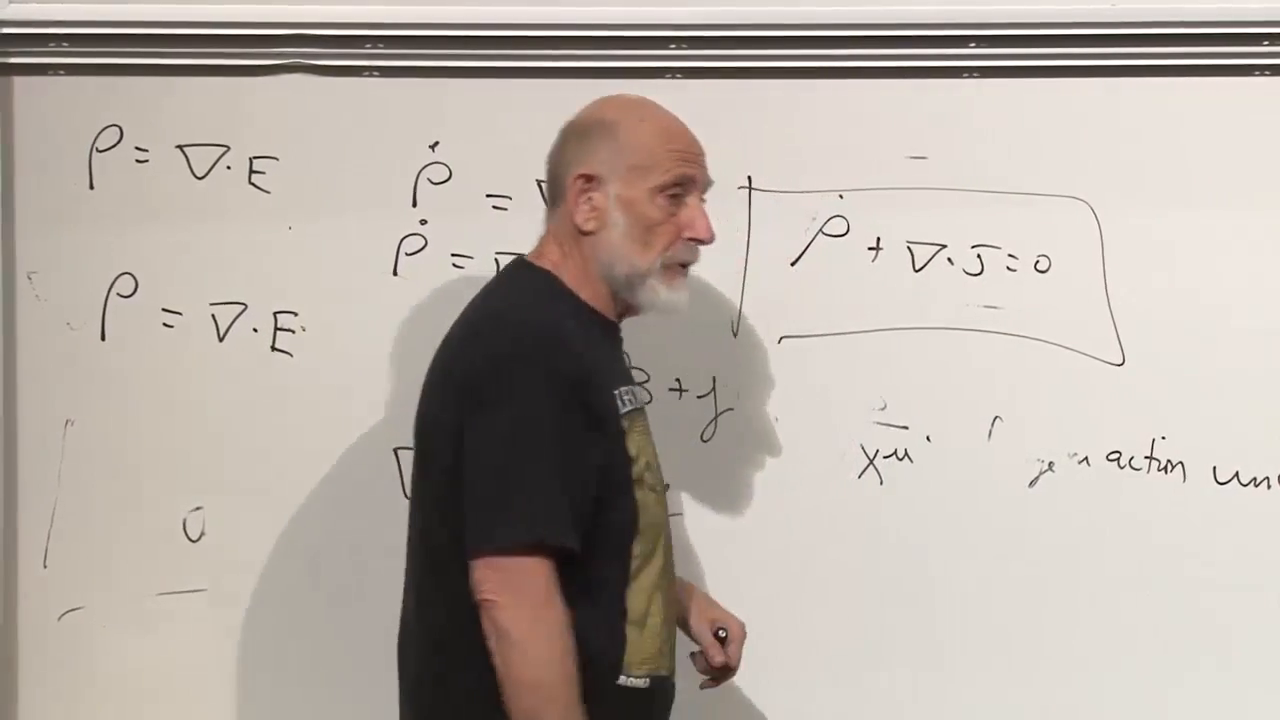
\includegraphics[width=\linewidth]{../../figures/lecture_09_figure_24.png}
\caption{The corrected source sign and the recovered continuity equation.}
\par\smallskip
\textit{Lecture frame: 01:31:00.}
\end{figure}

\begin{classroomqa}
\audiencequestion{Should the current term on the right be
\(-\mathbf J\)?}
\lecturerresponse{Yes. With the field-tensor convention used throughout
the course, the spatial part of
\(\partial_\mu F^{\mu\nu}=J^\nu\) is
\(\dot{\mathbf E}+\nabla\times\mathbf B=-\mathbf J\).
That correction makes the divergence calculation reproduce
\(\dot\rho+\nabla\cdot\mathbf J=0\) and does not alter the preceding
covariant action derivation. \lecturetimestamp{01:30:17}}
\end{classroomqa}

\section{Which Principle Is Fundamental?}

\begin{classroomqa}
\audiencequestion{Is the reasoning circular? We used charge
conservation to make the action gauge invariant, then used the action to
derive Maxwell's equations, and Maxwell's equations imply charge
conservation.}
\lecturerresponse{The statements are mutually compatible, not a circular
proof that assumes its own conclusion. One may begin with observed
Maxwell equations and discover the continuity equation; then
\(-J^\mu A_\mu\) is recognized as a gauge-invariant coupling. Or one may
begin with locality, Lorentz invariance, gauge invariance, and an action;
gauge invariance requires a conserved current and the action yields
Maxwell's equations. Or one may regard the physical fact that charge
does not disappear locally as primary. Each route reaches the same
structure. \lecturetimestamp{01:31:11}}
\end{classroomqa}

If one asks for the most economical constructive route, the combination
of locality, Lorentz invariance, gauge invariance, and a Lagrangian
principle selects
\begin{equation}
-\frac14F_{\mu\nu}F^{\mu\nu}-J^\mu A_\mu
\end{equation}
and hence Maxwell's dynamical equation. Calling one entry in this
triangle more fundamental is partly a matter of taste. The important
fact is that the entries fit.

\section{Why the Word \emph{Gauge}?}

\begin{classroomqa}
\audiencequestion{The mathematics is clear, but what does the word
\emph{gauge} mean here?}
\lecturerresponse{The name is a historical anachronism. A gauge can
refer to a chosen zero, as in pressure measured relative to a reference.
Hermann Weyl originally connected the idea to a local standard of length;
that interpretation was not the right physics. The term survived when
the freedom was correctly connected to the phase of a quantum wave
function. In the present classical calculation, changing
\(A_\mu\) by \(\partial_\mu\chi\) changes the descriptive zero without
changing \(F_{\mu\nu}\). The deeper quantum meaning is deferred.
\lecturetimestamp{01:34:49}}
\end{classroomqa}

The historical label should not obscure the operative statement:
potentials related by \eqref{eq:gauge-transform} describe the same
electromagnetic field. Gauge freedom is therefore a redundancy of the
potential description, while the field tensor is gauge invariant.

\section{Why the Two Maxwell Families Look Asymmetric}

\begin{classroomqa}
\audiencequestion{If electric and magnetic fields are so symmetric, why
does one Maxwell family appear as a Bianchi identity while the other
comes from equations of motion?}
\lecturerresponse{In source-free electromagnetism one may introduce a
dual potential so that the roles are exchanged: what was an equation of
motion becomes a Bianchi identity and vice versa. The physical
asymmetry enters through sources. Electric charges are observed, while
elementary magnetic monopoles have not been observed. If there were an
exact ordinary symmetry exchanging electric and magnetic charges, one
would expect magnetic counterparts with corresponding spectra, which
are not seen. More sophisticated theories can still contain magnetic
charges or electric--magnetic dualities, but that is beyond the present
derivation. \lecturetimestamp{01:37:11}}
\end{classroomqa}

Thus the source-free equations possess an electric--magnetic interchange
structure, while the observed source sector chooses an electric
description. That is more than a typographical convention, but it does
not invalidate the symmetry visible in a free plane wave.

\section{What Has Been Assembled}

The route through the lecture is now complete:
\begin{enumerate}
\item Maxwell's equations force a plane wave to be transverse, with
      orthogonal electric and magnetic fields and dispersion
      \(\omega=ck\).
\item The Bianchi equations are identities following from the potential;
      the contracted equations are dynamical.
\item Locality and Lorentz invariance lead us to an action density, while
      gauge invariance rules out \(A_\mu A^\mu\) and selects a scalar made
      from \(F_{\mu\nu}\).
\item The free action
      \(-\tfrac14F_{\mu\nu}F^{\mu\nu}\) yields the vacuum Maxwell
      equation.
\item The interaction \(-J^\mu A_\mu\) is gauge invariant exactly when
      the current obeys the continuity equation.
\item The sourced action yields
      \(\partial_\mu F^{\mu\nu}=J^\nu\), and antisymmetry gives
      \(\partial_\mu J^\mu=0\) back.
\end{enumerate}

This is a large amount of structure: Lagrangian mechanics, relativistic
field theory, electrodynamics, Lorentz invariance, gauge invariance, and
local charge conservation have become parts of one argument. The only
reliable way to digest it is to start again with the equations and carry
each derivative and sign through by hand.
